\chapter{Bullet Physics}

Bullet Physics é uma biblioteca livre para uso comercial escrita na linguagem de programação C++. É capaz de detectar e resolver a colisão entre objetos, interações entre articulações, além de simulações de tecidos e fluídos (BULLET, 2015).

A biblioteca é estruturada para ser utilizada como um todo ou apenas em parte. Pode-se utilizar somente a função de detecção de colisão, apenas o componente de \textit{rigid body} ou \textit{soft body} separadamente, ou mesmo somente a biblioteca de cálculos.

\begin{figure}[H]
	\centering
	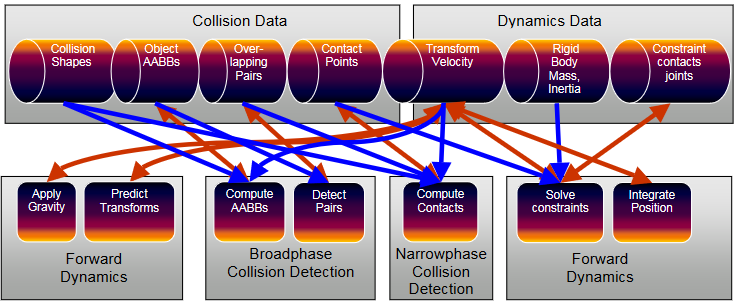
\includegraphics[scale=0.7]{imagens/bullet-pipeline.png}
	\caption{\small \textit{Pipeline} Bullet Physics (Fonte: BULLET, 2015)}
	\label{fig:bulletpipeline}
\end{figure}

A figura \ref{fig:bulletpipeline} apresenta os passos executados na implementação padrão, chamada de \lstinline{btDiscreteDynamicsWorld}, e onde são utilizados alguns objetos da biblioteca.

\section{Detecção de colisão}

Um dos recursos da biblioteca é a detecção de colisão. Na \textit{broadphase}, ou fase ampla, um algoritmo simples é executado para separar objetos que podem se colidir ou estão em colisão de objetos que não podem se colidir, seja porque estão parados ou muito distantes entre si. Posteriormente será executado um algoritmo mais complexo para definir as interações entre objetos colidindo.

Tais objetos são definidos por \lstinline{btCollisionObject}, que contém suas coordenadas e orientação, além de sua forma de colisão. Uma vez que as formas primitivas possuem algoritmos de colisão mais simples, é aconselhável utiliza-las sempre que possível. A figura \ref{fig:collisionshapes} demonstra a aplicação da esfera, caixa, forma convexa e malha de triângulos, respectivamente. Existem outras formas como cilindro, cone, cápsula, forma côncava e planos.

\begin{figure}[H]
	\centering
	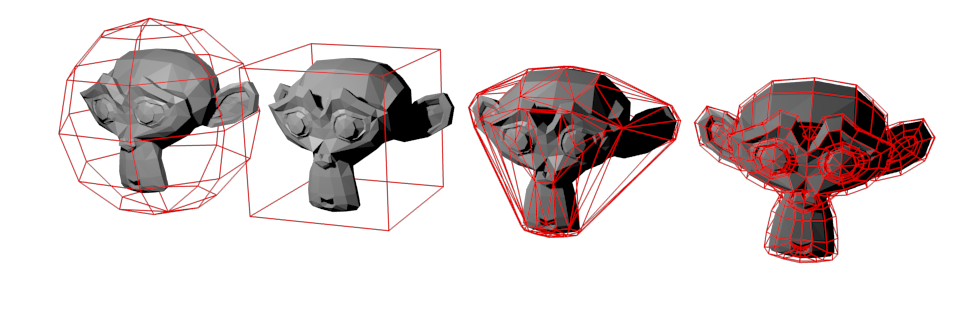
\includegraphics[scale=0.4]{imagens/collision-shapes.png}
	\caption{\small Diferentes formas de colisão aplicadas (Fonte: opengl-tutorial, 2017)}
	\label{fig:collisionshapes}
\end{figure}

\section{Dinâmica de corpos rígidos}
Corpos rígidos são definidos como um corpo composto de partículas que permanecem a distâncias fixas umas das outras ao longo do tempo. Representam boa parte dos objetos, com exceção corpos que se deformam, como tecidos e líquidos.

Na Bullet Physics é definida por um objeto \lstinline{btRigidBody}, que contém as propriedades necessárias para simular um corpo rígido, como fricção, restituição, velocidade linear e angular. Tais corpos podem ser estáticos, dinâmicos ou \textit{kinematic}. Objetos estáticos possuem massa infinita, declarada como zero na \textit{engine}, não se movem mas podem colidir. Objetos dinâmicos possuem massa positiva e têm sua posição atualizada a cada passo da simulação. Objetos \textit{kinematic} possuem massa infinita e têm sua posição controlada pelo sistema, não pela Bullet.

Para a fazer a interface entre o programa e o modelo físico pode se utilizar de um \textit{motion state}. Através dele a Bullet comunica as alterações nos objetos para que o programa atualize. No caso dos objetos \textit{kinematic}, o funcionamento é inverso: o programa atualiza a Bullet das atualizações feitas para que a biblioteca possa efetuar os cálculos. O método \lstinline{getWorldTransform} retorna um \lstinline{btTransform} com a posição e rotação atualizada do objeto.